\documentclass[11pt,a4paper]{report} 

% Für doppelseitigen Ausdruck (nur bei > 60 Seiten sinnvoll)
% \usepackage{ifthen}
% \setboolean{@twoside}{true}
% \setboolean{@openright}{true} 

\usepackage[german]{babel} % deutsch, deutsche Rechtschreibung
\usepackage[utf8]{inputenc} % Unicode-Zeichensatz als Text-Quelle
\usepackage[T1]{fontenc} % Umlaute und deutsches Trennen
\usepackage{mathptmx} % Times New Roman, gewohnter Font
\usepackage{courier} % einen schickeren Schreibmaschinenfont
\usepackage[scaled=.95]{helvet} % was serifenloses, wenn gebraucht
\usepackage{graphicx} % wir wollen Bilder einfügen
\usepackage{xfrac} % schöne Brüche im Fließtext mit sfrac
  
\usepackage{listings} % Schöne Quellcode-Listings [minted wäre besser]
\lstset{basicstyle=\sffamily, columns=[l]flexible, mathescape=true, 
  showstringspaces=false, numbers=left, numberstyle=\tiny}
\lstset{language=python} % und nur schöne Programmiersprachen ;-)
% und eine eigene Umgebung für Listings
\usepackage{float} % eigene Fließobjekte, kommen an beliebigen Stellen vor
\newfloat{listing}{htbp}{scl}[section] % Nummeriere je Abschnitt
\floatname{listing}{Listing} % listing ist ein Fließobjekt

% Auch wenn es anrüchig ist, man kann den Platz etwas mehr ausnützen
\usepackage[paper=a4paper,width=14cm,left=35mm,height=22cm]{geometry}
\usepackage{setspace}
\linespread{1.15} % nicht ganz anderthalbzeilig, nur ein bisschen mehr Platz
\setlength{\parskip}{0.5em} % kleiner Paragraphen(Absatz)-abstand
\setlength{\parindent}{0em} % im Deutschen Einrückung nicht üblich

% Seitenmarkierungen 
\usepackage{fancyhdr} % Schickere Header und Footer
\pagestyle{fancy}
% Zeichensatz für Header/Footer
\newcommand{\phv}{\fontfamily{phv}\fontseries{m}\fontsize{9}{11}\selectfont}
\fancyhead[L]{\phv HSMA Infos und Meinungen} % Kurztitel links oben
\fancyhead[R]{\phv \thepage} % rechts oben die Seitenzahl
\fancyfoot[L]{\phv Hochschule Mannheim} % Institution links unten
\fancyfoot[C]{\ } % keine Seitenzahl unten Mitte
\fancyfoot[R]{\phv Angewandte Prokrastination} % Studiengang rechts unten

\usepackage{url} % wir wollen eine URL anzeigen

 % alle Pakete und Einstellungen

%\bibliography{online}

% Hier anpassen 
\newcommand{\welchethesis}{Bachelor}
% \newcommand{\welchethesis}{Master}
\newcommand{\thesisofwas}{of Science}
\newcommand{\studiengang}{Technische Informatik}
% \newcommand{\studiengang}{Medizintechnik}
\newcommand{\titel}{Smartphones als Sensorbox}
\newcommand{\kurztitel}{Template Abschlussarbeit}
\newcommand{\autor}{Marius Cerwenetz}
\newcommand{\datum}{08. Juli 2022} % Abgabedatum
\newcommand{\ort}{Mannheim}
\newcommand{\referent}{Prof.\ Dr.\ Peter Barth}
\newcommand{\korreferent}{Prof.\ Dr.\ Jens-Matthias Bohli}

\begin{document}
\begin{titlepage}
  % Kopf der Seite
  \hsmalogo[1] \hfill
  \parbox[b]{60mm}{
    % \textsf würde das Aussehen der ersten Seite ruinieren, 
    % wer will, soll das selbst außen rum machen...
    Fakultät Informationstechnik\\
    Studiengang \studiengang}
  \begin{center}
    % rumfiddeln, damit es für 4 Zeilen gerade noch so geht...
    \rule{1\textwidth}{1pt}\\[-3mm]
    \parbox[t][64mm]{110mm}{% 11 cm für Breite 13, ca. 7 für Höhe 6
      \begin{center}
        \Large{\welchethesis arbeit}\\[2mm]
        {\begin{spacing}{1.13} \huge \bfseries \titel \end{spacing}}
        \vfill
        \Large{\autor} \\[1mm] % keep space to window
        \ 
      \end{center}
    }
    \rule{\textwidth}{1pt}    
    \vfill    
    {\Large Abschlussarbeit} \\[5mm]
    {\large zur Erlangung des akademischen Grades} \\[5mm]
    {\large \welchethesis\ \thesisofwas} \\[5mm]
    \vfill    
    \begin{tabular}{ll} % Mitte der Seite
      Vorgelegt von & \autor \\
      am & \datum \\
      Referent & \referent \\
      Korreferent & \korreferent
    \end{tabular}    
    \vfill
  \end{center}
\end{titlepage}
\cleardoublepage


% Erklärung gemäß der Prüfungsordnung
\thispagestyle{empty}
\subsection*{Schriftliche Versicherung laut Studien- und Prüfungsordnung}

Hiermit erkläre ich, dass ich die vorliegende Arbeit selbstständig verfasst
und keine anderen als die angegebenen Quellen und Hilfsmittel benutzt habe.

\vspace{6em}
\noindent\begin{tabular}{p{0.37\textwidth}p{0.56\textwidth}}
\ort, \datum  & \rule{0.56\textwidth}{0.5pt}\\
              & \makebox[1cm]{\ } \autor
\end{tabular}

\vfill

\cleardoublepage

 % Titelseite, Erklärungen, etc.

\begin{abstract}
In dieser Arbeit wurde ein Framework erstellt um Smartphonesensoren über eine Programmierumgebung auszulesen und Ausgaben auf dem Smartphone auszuführen.
Hierfür wurde eine Android-Anwendung, eine Kontrollanwendung und drei Softwarebibliotheken in dem Sprachen C, Java und Python implementiert.
Als Verbindungstechnologien kommen UDP und MQTT zum Einsatz.
\end{abstract}

\tableofcontents

\chapter{Einführung} \label{chap:intro}
Ziel dieser Arbeit ist es ein Framework zu entwickeln, dass Smartphones von Anwendern in eine Programmierumgebung einbindet um Sie beim Programmierenlernen zu unterstützen.
Hierbei stehen insbesondere die Interaktivität in Form von Sensordatenübermittlung und Ausgaben im Vordergrund.
\\\
Viele frische Entwicklerinneren und Entwickler oder Personen die das Programmieren gerade erst entdecken mühen sich zu Anfang mit grundlegenden softwaretechnischen Konzepten, syntaktischen Herausforderungen oder finden sich wieder in semantischen Stromschnellen.
Rein virtuelle, akademische Übungsaufgaben senken meist die Lernmotivation, abstrahieren gelerntes und lassen Softwareentwicklung fade und dumpf erscheinen.
Projekte mit Microcontrollern bieten eine praktikablere, einfache, realitätsbezogene Einstiegsmöglichkeit.
Spielerisch können kleine Projekte realisiert werden die durch physische Äußerungen Entwickler einladen sich an Problemen auszuporbieren.
Diese Eigenschaften sind insbesondere bei Projekten mit wenig Vorwissen für Lernwillige wie Schüler oder Erstemester-Studierende sinnvoll.
Gelerntes kann direkt angewand werden und Änderungen an Algorithmen sind schnell in der Verhaltensweise der Hardware erkennbar.
Praktische Programmieraufgaben bieten für Programmieranfänger den höchsten Lerneffekt bei höchster Motivation.\cite{learning_computer_programming}
\\
Die in Microcontroller integrierte Sensoren bilden hierbei den Schlüsselstein zwischen Änderungen in der realen Welt und Auswirkungen im virtuellen Programm.
Für Nutzer erscheint ein Gerät bedienbar.
Änderungen der realen Umgebung wirken sich unmittelbar auf den geschriebenen Algorithmus aus.
Bei einem Fehlverhalten kann dieser angepasst werden, bis das gewünschte Verhalten vorliegt.
Die ständige Berührung und Formung des Algorithmus mindert Ängste vor Änderungen, schafft Routine und damit ein tieferes Verständnis, Context und Hintergrundwissen für Probleme.
\\\\
Projekte mit Microcontrollern sind jedoch auch mit Nachteilen und Einstiegsvoraussetzungen behaftet.
Ein Arduino-Einstiegskit kostet im internen Arduino-Shop im Juni 2022 87,90 € \cite{arduino_kit}.
Ein Großteil der Kosten entfällt zwar auf den eigentlichen Microcontroller, ein nicht unmittelbarer Teil jedoch auch auf Peripherie wie wie Breadboards, Verbindungskabel und Erweiterungsboards.
Neben zusätzlich verursachten Kosten setzen Sie außerdem gewisses Hintergrundwissen voraus.
Für die erstmalige Verwendung von Breadboards muss beispielsweise bekannt sein welche Ports wie verbunden sind, welche Konventionen es für Plus- und Minuspol gibt und welche Bauteile für die Benutzung überhaupt geeignet sind.
Dies stellt eine Einstiegshürde dar, die die eigentliche interaktive Lernerfahrung herauszögert und Ziele entfernt.
Einstiegshürden wie dies führen zu einem Motivationsverlust.
\\\\
Durch Smartphones lässt sich dieses Problem jedoch umgehen.
Moderne Fertigungsverfahren der Halbleitertechnik reduzieren die durchschnittliche Chip-Größe enorm.
Dies betrifft auch Sensoren.
Bauartbedingte Einschränkungen sind heute nicht mehr so wesentlich wie zu Anfang der Smartphone-Entwicklung.
Aktuelle Smartphones sind daher bereits mit zahlreichen Sensoren wie Lagesensoren, Gyroskop oder Näherungssensoren ausgestattet.
Diese sind zwar für die komfortable Alltagsnutzung des Geräts konzipiert, können jedoch ganz regulär in Anwendungen dediziert angesteuert und ausgelesen werden.
\\
Die elektrische Komponente konventioneller Microcontroller-Sets erlaubt außerdem einen Fehlgebrauch der im schlimmsten Fall in der Zerstörung von Komponenten enden kann und zusätzliche Kosten verursacht.
Projekte mit Smartphones reduzieren diese Komplexitätsebene.
Sämtliche Schaltkreise sind bereits intern verschaltet und durch die Qualitätssicherung der Smartphone-Hersteller von möglichen Hardwarefehlern weitgehendst geschützt.
\\
Ein weiterer Vorteil Smartphones statt Microcontroller zu verwenden liegt in der Verfügbarkeit.
Weltweit besaßen 2022 5,2 Mrd. Menschen ein Smartphone. \cite{smartphone_users}
Vor allem jüngere Menschen nutzen Smartphones.
Viele Kinder besitzen bereits mit 10 Jahren \cite{bitkom_smartphones} ein Smartphone.
Da ein Smartphone üblicherweise nicht nur für Programmieraufgaben, sondern auch für den Alltag verwendet wird, sind die Anschaffungskosten hier auch nicht auf einen einzigen Zweck gebunden.
\\\\
Zusammenfassend lässt sich konstatieren, dass Smartphones eine Alternative zu herkömmlichen Microcontroller-Sets darstellen.
Sie verursachen weniger Kosten und sind meistens schon in Gebrauch.
Durch Ihre eingesetzten Sensoren können Sie zuverlässig Umgebungseigenschaften quantisieren.
Sie haben eine höhere Prozessorenleistung, so dass auch rechenintensivere Aufgaben ausgelagert werden können.
Durch die Entwicklungsmöglichkeiten von Mobilen Anwendungen sind der Kreativität der Ausgabemöglichkeiten keine Grenzen gesetzt.
Neben üblichen Übertragungsschnittstellen wie USB bieten Sie häufig auch eine W-LAN und Bluetooth-Funktion die eine Ansteuerung über unterschiedliche Technologien einfach macht und autonomere, den Umgebungsansprüchen angepasste Nutzungsszenarien ermöglicht.
\\
Eine Einbindung von Smartphones mit Bordmitteln ist in den meisten Prgrammierumgebungen jedoch nicht vorgesehen.
Smartphones und Entwicklungsumgebungen bieten meist keine direkte Möglichkeit der Kopplung.
Auch gibt es Seitens der Smartphone-Betriebssystemhersteller keine standardisierten Ausgabemöglichkeiten.
Moderne Smartphone-Betriebssysteme bauen sich modular aus mobilen Anwendungen auf, so dass das Betriebssystem keine direkten Ausgabemöglichkeiten besitzt.
Visuelle und haptische Ausgaben sind nur über mobile Anwendungen möglich.
\\
Das zentrale Thema besteht darin eine Smartphone-Anwendung für visuelle Ausgaben und Sensorwerte zu entwickeln und Schnittstellen in Programmierumgebungen zu schaffen, die die Nutzungsmöglichkeiten des Smartphones in Programmierprozesse einbinden.
Möglich wird dies durch Softwarebibliotheken die Funktionsaufrufe bereitstellen, welche Aktionen auf dem Smartphone auslösen.
Das Smartphone reagiert auf die empfangen Anfragen und führt die entsprechenden Kommandos aus.
Das Framework besteht aus einer programmiersprachenunabhängigen Bibliothek, einer Server-Anwendung und einer mobilen Anwendung für Android Smartphones.
Neben den technisch Details und Funktionsweisen werden in dieser Arbeit außerdem Beispielaufgaben gereich mit den angehende Programmiererinnen oder Programmierern gereicht.
Diese sind in Kapitel \ref{chap:Experimente} zu finden.
In Kapitel \ref{chap:architektur} werden die verwendeten Komponenten vorgestellt und Designentscheidungen innerhalb des Entwicklungsprozesses erläutert.
Die einzelnen Komponenten werden anschließend in Kapitel \ref{chap:app}, Kapitel \ref{chap:server_software} und Kapitel \ref{chap:libs} im Detail erklärt.
Zum Schluss werden die Ergebnisse in Kapitel \ref{chap:eval} vorgestellt und in Kapitel \ref{chap:fazit} diskutiert.


\chapter{Smartphones als Aktor und Sensor} \label{chap:Experimente}
Smartphones sind in sich geschlossene technische Geräte, die neben vordefinierten Verbindungsschnittstellen wie einem USB-Port, WLAN und Bluetooth meistens keine weiteren Schnittstellen bieten um externe Hardware und Schaltungen anzuschließen und Fernzusteuern.
Microcontroller-Schaltungen zum Programmierenlernen bieten meistens mehrere Ausgabemöglichkeiten wie LEDs, Lautsprecher oder Piepser.
Smartphones bestechen hier durch den Vorteil der virtuellen Darstellung auf dem Display.
Gewohnte Ausgabeelmente können dadurch virtualisiert werden.
Die Funktionen sind hier außerdem nicht nur von Mehrzweck-Ausgaben wie LED-Grids begrenzt die zum Beispiel für die Textanzeige oder Bildanzeige verwendet werden können.
Spezifische Zweckgebundene Elemente wie Textfelder, Textausgaben oder Bildausgaben in der App können beliebig kombiniert werden.
Darüber hinaus ist die Anordnung der jeweiligen Elemente frei, so dass das Layout anders als bei Microcontrollern auch im Nachhinein noch geändert werden kann, was den Entwicklungsprozess deutlich beschleunigt und flexibler macht.
\\
Moderne Smartphones bieten außerdem eine manigfaltige Menge an unterschiedlichen Sensoren.
Android bietet für die Verwendung Lage-, Temperatur-, Schwerkraft-, Licht-, Magnetfeld, Luftfeuchtigkeitssensoren und noch einige Weitere \cite{sensoren_android}.
Moderne Flaggschiff-Smartphones bieten viele dieser Sensortypen auch an.
Die Vielfalt übersteigt meistens die 
\\
Ein Nachteil liegt in der Ansteuerung von mechanischen Bauteilen wie Motoren.
Diese werden meistens durch eine elektrische Verbindung zwischen Bauteil und Controller realisiert.
Smartphones bieten diese Art der Ansteuerung nicht, da Hardwareschnittstellen wie GPIO-Pins nicht zur Verfügung stehen.
\\
Nichtsdestotrotz bieten Smartpones eine Menge Einsatzmöglichkeiten um einfache Programmierbeispiele auszuprobieren.
In diesem Kapitel werden in Abschnitt \ref{sec:activities} Beispielaufgaben für Programmiererinnen und Programmierer vorgestellt die Sie mit dem Framework lösbar sind.
Durchführbar ist dies durch verschiedene Ansteuerungen aus der Programmierumgebung der Entwickler.
Die einzelnen Ansteuerungen und Kommandos werden in Abschnitt \ref{sec:API} vorgestellt und erläutert.
Die Angebotenen Funktionalitäten stellen Anforderungen and das Projekt auf die in Abschnitt \ref{sec:anforderungen} eingegangen wird.

\section{Beispielprogrammieraufgaben}\label{sec:activities}
Praxisnahe Programmieraufgaben sollen angehende Softwareentwickler an Probleme heranführen.
Sie sollen nicht zu kompliziert, jedoch auch nicht zu trivial sein.
Unterschiedliche Schwierigkeitsklassen helfen ihnen sich selbst an Aufgaben heranzutasten.
Da die Aufgaben außerdem interaktiv gestaltet sein müssen sind Sie immer mit einem Äußeren Einfluss verbunden, auf den reagiert werden muss.
\\
Eine Liste der Aufgaben ist Tabelle \ref{tab:excercises} zu entnehmen.
\begin{table}[htbp]
  \centering
  \begin{tabular}{|l|c|c|c|}
      \hline
      Name der Aufgabe & Sensoren & Ausgaben & Schwierigkeit \\
      \hline
      Disco & - & Led & + \\
      \hline
      Würfeln & Lagesensor & Textfeld &+ \\
      \hline
      Diebstahl-Alarm & Näherungssensor & Textfeld, Led, Vibration & ++ \\
      \hline
      Klatsch-Zähler & Mikrofon & Textfeld & ++ \\
      \hline
      Dreh-Zähler & lagesensor & Textfeld & +++ \\
      \hline
  \end{tabular}
  \caption{Aufgaben}
  \label{tab:excercises}
\end{table}
Beschrieben wird der Name der Aufgabe, die benötigten Sensoren, die benötigten Ausgaben sowie der geschätzte Schwierigkeitsgrad.
Letzerer ist in drei größen gegliedert:
Einfach (+), Mittel(++) und Schwer (+++).
\\\\
In der Aufgabe \textit{Disco} soll eine virtuelle LED alle 500 ms die von der Farbe grün auf die Farbe rot wechseln.
Die Aufgabe benötigt keine Sensoren, da die LED nicht auf eine Eingabe seitens des Programmierers warten soll.
Sie soll immer blinken.
Die Ausgabe der farbig blinkenden LED wird über eine virtuelle LED auf dem Display des Smartphones realisiert.
Der Schwierigkeitsgrad ist als einfach einzustufen, da hier weder Sensoren benötigt werden, noch sonstige Abhängigkeiten innerhalb des Codes zu berücksichtigen sind.
\\\\
In der Aufgabe \textit{Würfeln} soll gemessen werden, ob ein Smartphone geschüttelt wurde.
Ist dies der Fall soll eine Zufallszahl generiert werden.
Anschließend soll diese auf dem Smartphone ausgegeben werden.
Verwendet wird dabei der Lagesensor, der Beschleunigungen in drei Achsenrichtungen misst.
Als Ausgabe muss für die Zufallszahl das Textfeld verwendet werden.
Die Schwierigkeit wird hier auch auf Einfach eingeschätzt, da lediglich ein Sensor und eine Ausgabe verwendet wird.
Auch der Algorithmus ist nicht von vielen Abhängigkeiten geprägt.
\\\\
In der Aufgabe \textit{Diebstahl-Alarm} soll überprüft werden, ob der Näherungssensor eine Annäherung gemessen hat.
Wenn dies der Fall ist soll der Text \glqq ALARM\grqq{} auf dem Smartphone ausgegeben werden.
Das Smartphone soll fünf mal für die Zeit von 1000ms vibrieren.
Die Farbe der virtuellen LED soll wie in Aufgabe \textit{Disco} alle 500ms die Farbe wechseln.
Dies soll einen Diebstahl-Alarm simulieren bei der sich jemand mit der Hand dem Smartphone nähert.
\\
Hier wird lediglich der Näherungssensor verwendet um eine Näherung zu detektieren.
Die Ausgabe des Alarm-Textes soll auf einem Textfeld dargestellt werden.
Außerdem sollen die Vibrationsmotoren des Smartphones, die sonst beispielsweise für Benachrichtigungen verwendet werden, benutzt werden um ein haptisches Feedback zu liefern.
Der Schwierigkeitsgrad der Aufgabe ist als \textit{Mittel} eingestuft, weil die Aufgabe zu unterschiedlichen Zeit, unterschiedlich lang auf mehreren Ausgabemöglichkeiten erfolgen muss.
Außerdem ist die Ausgabe an die Bedingung einer Näherung an das Smartphone gebunden.
\\\\
Bei der Aufgabenstellung \textit{Klatsch-Zähler} muss für einen definierten Zeitraum die Anzahl der Klatscher gemessen werden.
Programmierer starten also ein Programm und klatschen vor dem Smartphone in die Hände.
Die Anzahl der Klatscher soll dann gemessen und auf dem Display des Smartphones ausgegeben werden.
Verwendet wird dafür lediglich das Mikrofon und das Textfeld des Smartphones.
die Schwierigkeit ist hier ebenfalls auf \textit{Mittel} gesetzt, da die Klatscher auf den Sensor nicht immer die gleiche intensivität haben.
Programmierer müssen also erproben, wann es sich wirklich um ein Händeklatschen handelt und wann einfach nur Hintergrundgeräusche zu hören sind.
\\\\
Bei der Letzen Aufgabe \textit{Drehzähler} soll der Programmierer das Smartphone innerhalb eines eigens definierten Zeitraums drehen und anhand der zurückgegeben Werte die Anzahl der Drehungen ermitteln.
Diese soll anschließend im Textfeld auf dem Smartphone ausgegeben werden.
Zur Verwenung kommen hier ebenfalls der Lagesensor als Sensoreingabe und das Textfeld als Ausgabe.
Die Aufgabe ist als \textit{Schwer} bewertet, da hier Wiederholungen in einer Werteabfolge erkannt werden müssen.
Diese sind jedoch nicht immer exakt gleich.
So muss auch erprobt werden wie sich eine Umdrehung überhaupt in den Werten äußert und wie Drehungen optimal erkannt werden können.
\\\\
Die Aufgaben können natürlich nach Belieben kombiniert werden.
\textit{Disco} ist beispielsweise schon in \textit{Diebstahl-Alarm} integriert.
Denkbar wäre auch beim \textit{Wüfeln} den \textit{Klatschzähler} für die generierung der Zufallszahl zu verwenden.
Der Diebstahlalarm kann auch bei einer ungeraden Anzahl an Drehungen des Drehzählers gestartet werden.
\\
Dadurch werden Programmierern Konzepte wie Schleifen oder Bedingungen nah gebracht.
Zum Beispiel könnte die LED blinken wenn eine gewisse Umdrehungsanzahl erreicht wurde um While-Schleifen zu erläutern.

\section{Funktionsaufrufe}\label{sec:API}
Gelöst werden sollen die Aufgaben durch das Aufrufen der API.
Diese bietet die benötigten Funktionen an.
Die Aufrufe sind frei miteinander kombinierbar, so dass Aufgaben erweitert werden können.

\section{Softwareanforderungen}\label{sec:anforderungen}
Aus den unter \ref*{sec:API} genannten Funktionen ergeben sich die Anforderungen an das Framework.
\\
Es wird unterschieden in Funktionen die Sensordaten auslesen und Funktionen die Aktionen auf dem  auslösen.
\section{Sensordaten-Funktionen}
Um das optimale Lernergebnis zu erhalten müssen Sensordaten responsiv vorliegen.
Je schneller Richtungs-, Helligkeits oder Lautstärkedaten vorliegen desto schneller kann im Programm drauf reagiert werden.
So können Experimente eher begriffen werden, da Auswirkungen in der Realität instantan Auswirkungen auf den vom Schüler geschriebenen Programmablauf haben.
Eine maximale Responszeit von ca. 20 ms ist hierfür zielführend.
\\
Beim Aufruf der Funktion wird kein Aufruf gestartet der das Smartphone anweist eine einzelne Sensormessung zu starten und den aktuell vorliegenden Sensorwert zurückzusenden.
Die Latenzen zwischen Smartphone und Bibliothek könnten je nach Verbindungsart, Bandbreite und Geräteanzahl im WLAN stark varrieren.
Das Smartphone muss in periodischen Abständen Sensordaten messen und senden. Die Sensorwerte werden dann zentral auf dem gleichen Rechner, auf dem auch die Bibliothek läuft zwischengespeichert.
So wird die mögliche Distanz zwischen Sender und Empfänger beschränkt auf den gleichen Rechner.
Sensordaten liegen immer zwischengespeichert vor.
Neue Daten werden beim Eintreffen der periodischen Aktualisierungen eingetragen.
Ein Funktionsaufruf der Sensordaten abfragt muss dann auf die zentral zwischengespeicherten Sensordaten zurückgreifen.
So wird der Responszeit erhöht und es liegt immer das aktuellste Sensor-Ergebnis im Zwischenspeicher vor.
Der Tätigkeitsbereich vom Smartphone umfasst jedoch nicht nur die Messung und Übermittlung der gemessenen Daten.

\section{Auslösende Funktionen}
Die Anwendung auf dem Smartphone bietet ebenfalls verschiedene UI-Elemente welche aus der Ferne per Funktionsaufruf bedient werden.
Außerdem werden zeitlich beschränkte Messungen umgesetzt die auf Anfrage gestartet werden sollen.
Diese Art der Aufrufe benötigt keinen kontunierlichen Strom aus Werten, sondern wird einzeln aufgerufen und geben gegebenenfalls einzeln Werte zurück.
Der Fokus liegt bei diesen Anfragen nicht auf Responsivität, sondern auf Sicherheit des Aufrufs.
Bei dieser Art Aufruf werden Daten erst auf Anfrage generiert und dann, sofern vorgesehen, zurückgesendet.

\

\chapter{Architektur} \label{chap:architektur}
Der Aufbau des Frameworks besteht aus einer mobilen Anwendung für Android-Smartphones, Bibliothek in der Programmiersprache C und einer Middleware die den Austausch Koordiniert.
Der Aufbau ist in Abbildung \ref{fig:design} dargestellt.
\begin{figure}[htbp]
  \centering
  \includegraphics[width=.9\textwidth]{images/design.png}
  \caption{System-Aufbau}
  \label{fig:design}
\end{figure}
Clientseitig erfolgen sämtliche Aufrufe die Sensordaten abgreifen oder Steueranfragen senden immer erst per UDP über die Middleware.
\\
Die Middleware sammelt, sobald sich eine Android-Anwendung bei ihr anmeldet, gewisse Sensordaten und speichert Sie intern zwischen, damit Sie schnell vorrätig vorliegen.
Die Speicherung erfolgt in einem seperaten Thread, der die letzten Zustände der Sensordaten hält.
Werden Sensordaten abgerufen werden Sie aus der Liste entfernt.
Sind noch keine Daten vorhanden, oder wird ein Sensor angefragt der im Smartphone nicht existent ist, wird ein Fehlercode zwischengespeichert.
Die Verfügbarkeit der jeweiligen Sensoren wird beim Start der Anwendung ermittelt.
\\
Steueraufrufe werden beim Aufruf über ein seperates Topic versandt.
Der Austausch erfolgt auf mehreren Topics, da manche Nachrichten, wie Steuerbefehle wie in \ref{subsec:Ausgaben} erwähnt, mit einem höheren QOS-Level versendet werden müssen als im Moment existente Sensordaten die nur eine kurzzeitige Relevanz besitzen und deren Zustellung nicht obligatorisch ist.
Auf diesem Topic werden Nachrichten mit der QOS von 2 versandt auf dem für reguläre Sensordaten mit einer QOS von 0.
% Todo: admin channel? Erster Aufbau auf admin channel mit anschließender negotiation auf welchen channeln gesendet werden soll. Wie hart aufziehen?

\section{Nachrichtenformate}
Damit der gesamte Funktionsablauf des Frameworks korrekt funktioniert müssen Nachrichten zwischen den einzelenen Komponenten ausgetauscht werden.
Hierfür wird ein Format definiert dass die in Kapitel \ref{sec:anforderungen} erwähnten Anforderungen sowohl auf Library-, Middleware-, und Smartphone-Seite umsetzt.

Die Nachrichten werden im JSON-Format übertragen.
Jede Nachricht beeinhaltet mindestens die Angabe eines Nachrichtenformat-Typs.
Für die Aufrufe wurden folgende Nachrichtenformate definiert:
\begin{enumerate}
  \item sensor\_request
  \item sensor\_update\_request
  \item rpc\_request
  \item rpc\_response
\end{enumerate}
Die Nachrichtenformate werden als Vorlagen in einer zentralen Datei abgelegt.
Diese werden in der Library, Middleware und auf dem Smartphone eingelesen, damit Sie nur einer Stelle definiert werden müssen, wie in \ref*{fig:all_json} dargestellt.
Neben den Nachrichtenformaten werden hier auch weitere Konfigurations-Konstanten wie Commands für rpc\_requests, Namen der Sensordaten und Namen der MQTT Topics spezifiziert spezifiziert.


\begin{figure}[htbp]
  \centering
  \includegraphics[width=.9\textwidth]{images/all_json.png}
  \caption{Zentrale Konfigurationsdatei}
  \label{fig:all_json}
\end{figure}


\textbf{sensor\_requests} werden vom Endanwender-PC per UDP an die Middleware gesendet.
Sie beeinhalten neben dem Typ das Feld \texttt{sensor\_type}.
Dieses definiert den Sensortyp für den eine Anfrage generiert wurde.
Eine Übersicht ist in Listing \href{lst:sensor_request} zu finden.
\\
Im Listing wurde der Platzhalter \texttt{TYPE} für alle möglichen Sensortypen angegeben.
Eine vollständige Aufschlüsselung ist in Tabelle \ref{tab:sensor_types} zu finden.
\lstinputlisting[label={lst:sensor_request}, caption={sensor\_request}, captionpos=b]{listings/messages/sensor_request.json}

\textbf{sensor\_update\_requests} werden von Smartphone über MQTT an die Middleware versandt.
Sie umfassen ebenfalls wie \texttt{sensor\_requests} das Feld \texttt{sensor\_type}, jedoch zusätzlich auch das Feld \texttt{value} in dem der gemessene Sensorwert gespeichert wird.
Dieser wird von der Middleware in eine interne Datenstruktur eingetragen.

\textbf{rpc\_requests} werden vom Endanwender-PC per UDP an die Middleware gesendet.
Sie lösen Aktionen auf dem Smartphone aus wie zum Beispiel das anschalten der LED, oder das Starten von Messungen.
Sie werden von der Middleware per MQTT an das Smartphone weitergereicht.
Die Übermittlung erfolgt jedoch über ein seperates Topic mit einem Quality of Service Wert von 2 um eine garantierte Übertragung zu gewährleisten.

rpc\_requests und response beeinhalten außerdem mindestens ein \texttt{command}-Feld und ein \texttt{value}-Feld.

Nachfolgendes Listing zeigt beispielsweise den Aufruf die LED einzusschalten.

\lstinputlisting[]{listings/messages/led.json}
Folgende Nachricht beschreibt beispielsweise den übermittelten Sensorwert des accelerometers.
\lstinputlisting{listings/messages/accell.json}

\section{Nachrichtenablauf}

Der Nachrichtenablauf ist in Abbildung \ref{fig:message flow} dargestellt.
\begin{figure}[htbp]
  \centering
  \includegraphics[width=.9\textwidth]{images/message_flow.png}
  \caption{Nachrichtenablauf}
  \label{fig:message flow}
\end{figure}
\\
Grau dargestellt ist hier die periodische aktualisierung der Sensordaten durch sensor\_update\_requests.
Diese werden mit einer auf dem Smartphone definierten Taktung an die Middleware übertragen
Die Middleware trägt die neuen Daten dann in der internen Datenbank ein.
\\
Grün dargestellt ist der Ablauf eines sensor\_requests.
Aus der Library heraus werden sensor\_requests gesendet.
Die Middleware, die die aktuellen Sensorwerte vorhält sendet dann als Antwort den Sensorwert als einzelnen Wert, also nicht im JSON-Format zurück.
\\
Blau dargestellt ist ein rpc\_request, dass ein Command auf dem Smartphone ausführt, dass keinen Rückgabewert zurückliefert. Änlich wie bei sensor\_update\_requests handelt es sich hier um fire-and-forget-requests.
\\
Lila dargestellt sind rpc\_requests die ein Command ausführen dass einen Rückgabewert erwartet, wie es beispielsweise bei zeitlich getakteten Messungen der Fall ist. 
In diesem Fall wird eine rpc\_response-Nachricht mit versendet.



\section{Verwendete Technologien}\label{sec:net_tech}
In diesem Kapitel werden die Technologien und Protokolle beschrieben die beim Nachrichtenaustausch zwischen Library, Middleware und Smartphone zum Einsatz kommen.
\\
Der Fokus liegt auf Serialisierung und Transport.
Da im gesamten Prozess zwischen den drei Einheiten unterschiedliche Programmiersprachen auf verschiedenen Plattformen zum Einsatz kommen müssen sämtliche Protokolle und Notationen von möglichst vielen Programmiersprachen unterstztützt werden.
\\
Beim Transport liegt die Anforderung vor allem auf einer schnellen Ausführung, da sich Sensordaten schnell ändern und ein Lerneffekt am Besten eintritt wenn keine hohen Latenzen bei der Übertragung auftreten.

\section{JSON}
JSON ist eine Abkürzung für JavaScript Object Notation.
Es handelt sich um ein Nachrichten-Austausch-Format \cite{json}
\\\\
Der Aufbau ist minimalistisch. Objekte können mit Schlüssel-Wert-Paaren serialisiert werden.
Auch Arrays können eingesetzt werden.
Durch den einfachen Aufbau werden für eine Nachricht auch nicht viele Ressourcen benötigt.
Gerade bei der Übertragung von Sensordaten ist ein schneller Datenaustausch sehr positiv.
\\
JSON wird außerdem von vielen Programmiersprachen wie Python und Java nativ unterstützt.
Da die Bibliotheken programmiersprachenunabhäng bereitgestellt werden sollen bietet sich JSON als gemeinsame Notation hervorrangend an.
Da es in C keinen eingebauten JSON Parser gibt wird hier auf den cJSON \cite{cjson} zurückgegriffen.

\section{MQTT}
MQTT steht für Message Queuing Telemetry Transport und ist ein Client-Server Protokoll das auf TPC basiert.
Es kommt häufig mei Machine-to-Machine Interaktionen zum Einsatz.
Dies umfasst Lösungen im IoT-, Smarthome und Automatisierungstechnik-Bereich.
Durch den platzsparenden Header von 2 Bytes und einer maximalen Nachrichtengröße von ca. 260 MB ist es gleichzeitig ein leichtgewichtiges jedoch auch flexibles Protokoll zum Nachrichtenaustausch.
\\
Für den Nachrichtenaustausch registrieren sich Clients an einem Broker, dem MQTT-Server, an ein oder mehrere Topics.
Auf diesen Topics können dann Nachrichten gesendet und empfangen werden.
Topics können hierarchisch geschichtet werden.
Subtopics können dann pro ebene oder rekursiv für alle Subtopics abboniert werden.
Dieses Feature ist jedoch für die Entwicklung nicht weiter von Belang.
Nachrichten werden von Clients an den Broker gesendet.
Dieser hält den Nachrichteninhalt intern für das jeweilige Topic.
\\
Alle Clients besitzen einen Identifier, so dass empfangene Nachrichten zurückgeführt werden können.
Somit sind auch Topic-Interne Filter möglich nur Nachrichten von bestimmten Clients zu empfangen.
\\
Nachrichten können mit einer Quality of Service (QoS), einer Übertragungsgüte, übertragen werden.
Insgesamt gibt es drei Stufen: 0, 1 und 2.
Je höher die QoS-Stufe desto höher die Latenz der Übertragung.
\\
Bei einer QoS von 0 werden Daten einfach übertragen ohne sicherzugehen, dass die Nachricht auch wirklich beim Broker ankommt. 
Bei QoS 1 wird eine Nachricht so lange auf einem Topic gesendet bis der Broker den Empfang einmal bestätigt.
Es kann jedoch auch passieren, dass der Broker die Nachricht mehrmals empfängt und nur einmal bestätigt.
Bei QoS 2 wird die Nachricht einmal an den Broker gesendet.
Dieser muss dann den Empfang der Nachricht einmal bestätigen.
Erst dann gilt die Nachricht als Empfangen.
\\
Damit die verlangte Güte sichergestellt wird müssen Sender und Empfänger mit der gleichen Güte senden bzw. ein Topic mit der gleichen Güte-Stufe abbonieren.
Wird ein Topic mit einer geringeren Güte abboniert als die Güte der publizierten Nachricht wird die Nachricht mit der Güte des Abbonenten übertragen.
Wenn eine Nachricht mit geringerer Güte auf einem Topic publiziert wurde als dieses Topic abboniert wurde wird die Übertragung mit der Güte-Stufe des publizierenden Clients übertragen.

\section{UDP}
UDP ist ein verbindungsloses Netzwerkprotokoll, dass auf der Transportschicht des TCP/IP-Stack zum Einsatz kommt.







\chapter{Android Anwendung}\label{chap:app}
Die Android-Anwendung läuft auf dem Smartphone des Anwenders.
Sie besteht aus einer Haupt-Activity deren außerlicher Aufbau in Kapitel \ref{sec:androidApp} beschrieben ist. 
\\
In der Haupt-Activity wird ein Service gestartet und gebunden.
Der Service baut eine Verbindung zu einem MQTT Server auf.
Dort verbindet er sich den beiden Topics. 
Die Activity bindet beim Start den MQTT-Service ein.
Stellt ein Client über die Bibliothek auf einem Computer eine Anfrage wird dieser Aufruf, wie z.B. eine Ausgabe auf einem Textfeld an das Smartphones,  zuerst zur Middleware geleitet.
Diese leitet die Anfrage weiter an das Smartphone, dass dann den jeweiligen Befehl ausführt.
Dies beeinhaltet vor allem Ausgaben, sowie Eingaben die eine Nutzerinteraktion mit reduziertem Ergebnis.
Zum Beispiel alle Eingaben die etwas in einem angegebenen Zeitraum messen.
Falls ein Sensor angefragt wird der auf dem Smartphone nicht existiert wird eine Nachricht mit einer Fehlermeldung zurückgegeben.


\section{Kommandos und Ausgaben}
Für die Ausgabe auf dem Smartphone sind verschiedene Kommandos definiert.
Diese sind der Tabelle \ref{tab:command_types} zu entnehmen.
\texttt{CMD-Kürzel} beschreibt die Notation des Kürzels mit dem eine Aktion ausgeführt werden kann.
Diese wird unter \texttt{Beschreibung} kurz zusammengefasst.
\texttt{return} gibt an, ob der Aufruf des Requests eine Antwort rücksendet und somit auch, ob ein Aufruf der Funktion in der Library blockiert oder nur sendet.


\section{Sensoren}
Smartphones beeinhalten verschiedene Sensoren die Daten über die Umgebung erfassen können.
In der Android Anwendung werden folgende Sensortypen verwendet:
\begin{itemize}
  \item Lineare Beschleunigungssensoren
  \item Mikrofon
  \item Annäherungssensor
  \item Gyroskop
\end{itemize}

\section{Lineare Beschleunigungssensoren}
Beschleunigungs- bzw. Lagesensoren messen die Beschleunigung in $m/s^2$ für die drei Bewegungsrichtungen: X-, Y- und Z-Achse in einem festgelegten Zeitraum.
Eine Übersicht über die Anordungen der drei Axen ist in Grafik \ref{fig:and_axes} zu sehen.
\begin{figure}[htbp]
  \centering
  \includegraphics[width=.8\textwidth]{images/android_axes.png}
  \caption{Android-Koordinatensystem}
  \label{fig:and_axes}
\end{figure}
Die X-Achse verläuft horizontal durch das Display des Smartphones hindruch, die Y-Achse vertikal und die Z-Achse durchschneidet das Smartphone in die Tiefe.
\\\\
Die Frequenz mit der Messwerte erstellt werden kann manuell angegeben werden.
Hierfür stehen vier Schnelligkeitsstufen bereit.:
\begin{itemize}
  \item SENSOR\_DELAY\_FASTEST : Kein Verzögerung. Verwendet die Frequenz des Sensors.
  \item SENSOR\_DELAY\_GAME : Verzögerung um 1ms
  \item SENSOR\_DELAY\_UI : Verzögerung um 2ms
  \item SENSOR\_DELAY\_NORMAL : Verzögerung um 3ms
\end{itemize}
Die mit der jeweiligen Frequenz aufgenommenen Beschleunigungssensordaten beeinhalten jedoch auch die Ergbeschleunigung.
Diese muss für die bereinigten, realen Werte zuerst noch von den aufgenommenen Werten subtrahiert werden\cite{accel_g}.


\section{Angaben für die Nachrichtenformate}
Alle Sensordaten besitzen ein festgelegtes Kürzel zur Standardisierung des Nachrichtenverkehrs.
Sie dienen vor allem der Adressierung der jeweiligen Daten in der Middleware und in der Library.
\\
Die Sensortyp Kürzel sind in Tabelle \ref{tab:sensor_types} zu finden. 
\begin{table}[htbp]
  \centering
  \begin{tabular}{|c|c|c}
      \hline
      TYPE-Kürzel & Beschreibung \\
      \hline
      accell\_x & Lagesensor für die X-Richtung \\
      \hline
      accell\_y & Lagesensor für die Y-Richtung \\
      \hline
      accell\_z & Lagesensor für die Z-Richtung \\
      \hline
       gyro\_x & Gyroskopsensor für die X-Richtung \\
      \hline
      gyro\_y & Gyroskopsensor für die Y-Richtung \\
      \hline
      gyro\_z & Gyroskopsensor für die Z-Richtung \\
      \hline
      prox & Näherungssensor \\
      \hline

  \end{tabular}
  \caption{Sensor-Kürzel mit Beschreibung}
  \label{tab:sensor_types}
\end{table}


\chapter{Kontrollanwendung}\label{chap:server_software}

Für Vermittlung zwischen den Komponenten fungiert eine Server-Anwendung.
Sie ist in Python geschrieben und vermittelt zwischen UDP-Anfragen auf der einen Seite vom Client aus und MQTT-Anfragen vom Smartphone auf der anderen Seite.
User können über die Library RPC-Anfragen oder Sensor-Anfragen an den Server stellen.
Dies geschieht in form von JSON-Anfragen die per UDP übermittelt werden.
Der Server ist unter der localhost-Adresse 127.0.0.1 auf dem Port 5006 erreichbar.
\\
Für die MQTT-Verbindung kommt dabei die unter OpenSource-Liznenz stehende MQTT-Library Paho der Eclipse-Foundation zum Einsatz. \cite{paho}


\section{Anforderungen}
Aus den Anforderungen ergeben sich folgende Aufgaben die der Server umsetzen muss:
\begin{itemize}
\item Sensoranfragen schnell beantworten
\item Anfragen die Funktionen auf dem Smartphone starte, müssen schnell an das Smartphone weitergereicht und gegebenfalls wieder beantwortet werden.
\end{itemize}
Damit Sensoranfragen schnell beantwortet werden können, werden die aktuellen Sensorworte fortlaufend vom Smartphone an den Server übermittelt.
Dieser speichert Sie dann, sobald ein Sensorwert gemessen und übermittelt wurde in eine interne, threadsichere Datenstruktur.
Hierdurch wird insbesondere der Latenzunterschied zwischen Smartphone und Localhost berücksichtigt.
UDP Anfragen per Localhost haben eine wesentlich geringe Latenz als MQTT-Anfragen, auf die das Smartphone reagieren muss.
Durch das Cachen auf dem Server liegen bei Anfragen per UDP, also von der Library aus, immer Sensordaten vor.
\\
Um Funktionsanfragen zeitnah auszuführen müssen unterschiedliche Netzwerklatenzen berücksichtigt werden.
Die Übermittlung erfolgt asynchron zwischen Library und Smartphone, wobei zu erwarten ist dass Übermittlungen an das Smartphone mit einer höheren Latenz übertragen werden, als Anfragen zwischen Library und Server, da sich beide auf dem gleichen Host befinden.
Die Verbindung zwischen Library und Server erfolgt darüber hinaus über localhost und somit über ein Loopback-Device.
Loopback-Devices reichen Netzwerkpakete nicht herkömmlich über ein physisches Netzwerkinterface weiter sondern stellen ein virtuelles Gerät dar, dessen Übertragungsrate an die CPU gekoppelt ist.
Die Bandbreiten sind dadurch sehr hoch und die Latenzen gering.
\\
Um die Latenzen und die damit verbundenen unterschiedlichen Auftrittszeitpunkte von Anfragen zu berücksichten, sowie eine möglichst effiziente Abarbeitung der selbiger zu ermöglichen wird eien paralelle Algorithmusstruktur verwendet.

\section{Interner Aufbau}
Die Serveranwendung mit dem Namen server.py ist aufgeteilt in einen Datenverwaltungsteil, DataHandler, und eine MQTT Anbindung, MQTTHandlerThread.
Da die Sensorwerte des Smartphoens vorrätig gehalten werden, wird außerdem eine Datenklasse für diese, SensorDB, intern gehalten.
Eine Übersicht über die Komponenten ist Abbildung \ref{fig:serverUml} zu entnehmen.
\begin{figure}[htbp]
  \centering
  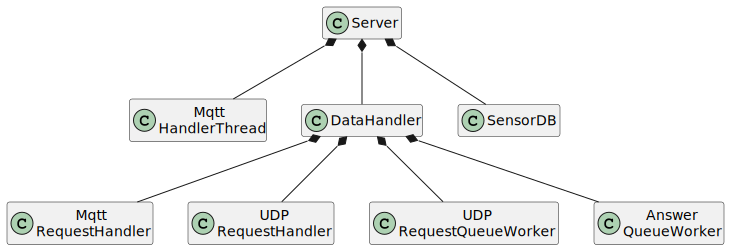
\includegraphics[width=.8\textwidth]{images/ServerUml.png}
  \caption{UML Digaramm Server}
  \label{fig:serverUml}
\end{figure}
\\
DataHandler wiederrum teilt sich nochmal auf in vier seperate Funktionen, die als Threads nebenläufig laufen: MqttRequestHandler, UDPRequestHandler, UDPRequestQueueWorker und AnswerQueueWorker.
\\
Die Funktionsweise und Zwecke dieser Threads wird im Folgenden an zwei Beispielen erläutert.
Für das erste Beispiel wird Abbildung \ref{fig:serverMqttReqPath} betrachtet.
Zu sehen ist ein MQTT-Request, also eine Anfragen des Smartphones, dass über MQTT an den Server gesendet wird.
Schnittstellen zu MQTT sind in der Grafik grün, Schnittstellen zur Library per UDP, sind blau markiert.
\begin{figure}[htbp]
  \centering
  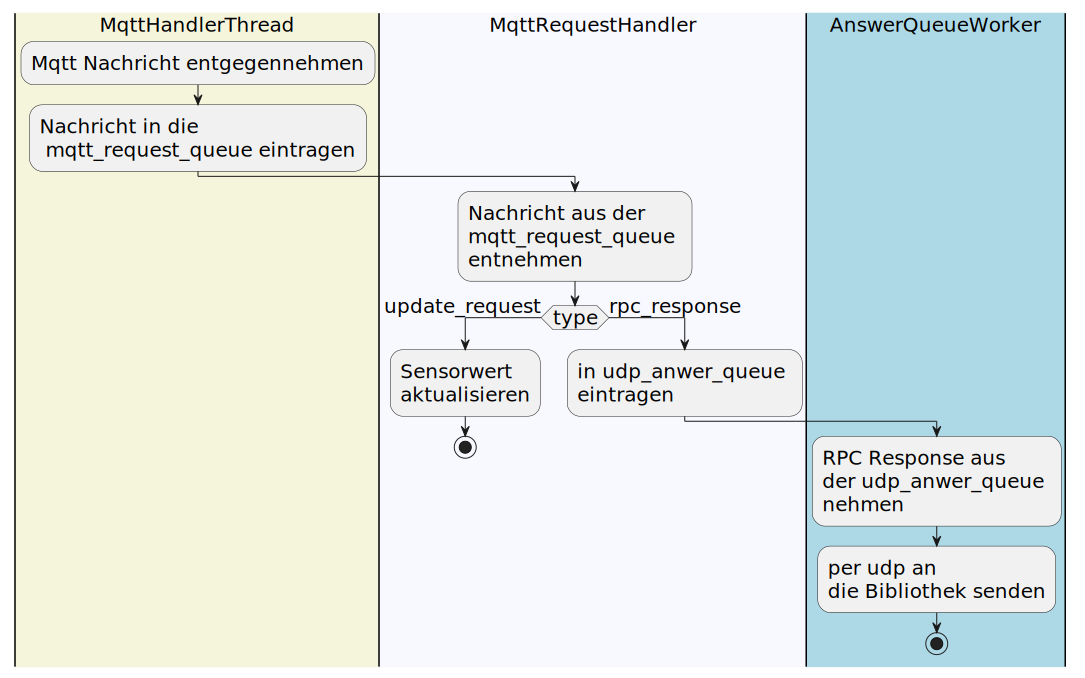
\includegraphics[width=.8\textwidth]{images/MqttRequestServerPath}
  \caption{Ablaufdiagramm MQTT Request}
  \label{fig:serverMqttReqPath}
\end{figure}
\\
Erreicht ein MQTT Request den Server wird es im MQTTHandlerThread entgegengenommen.
Dieser setzt die Nachricht in eine MQTTRequestQueue ein.
Der MQTTRequestHandler des DataHandlers wartet bis ein Eintrag in der Queue vorhanden ist und nimmt gegebenenfalls eine Nachricht.
Daraufhin wird derTyp des Requests bestimmt.
Handelt sich um ein Sensorupdate muss nur der Sensorwert in der Datenbank aktualisiert werden.
Handelt es sich um eine rpc\_response, also um eine Antwort auf eine vorausgegangenes rpc\_request, dass einen Rückgabewert fordert, wird das request in eine udp\_answer\_queue eingefügt.
Der AnswerQueue Worker wartet, ähnlich wie der MQTT Request Handler, bis eine neue Nachricht vorhanden ist die per UDP an den Client gesendet werden soll und sendet diese dann gegebenfalls ab.
\\

Das zweite Beispiel befasst sich mit dem Ablauf eines UDP-Requests, also einer Anfrage die mithilfe der Library gesendet wurde.
Der Ablauf ist in Abbildung \ref{fig:serverUDPReqPath} dargestellt.
Wie auch schon in der letzten Grafik sind alle Schnittstellen zum Smartphone grün und alle Schnittstellen zur Library blau markiert.
\begin{figure}[htbp]
  \centering
  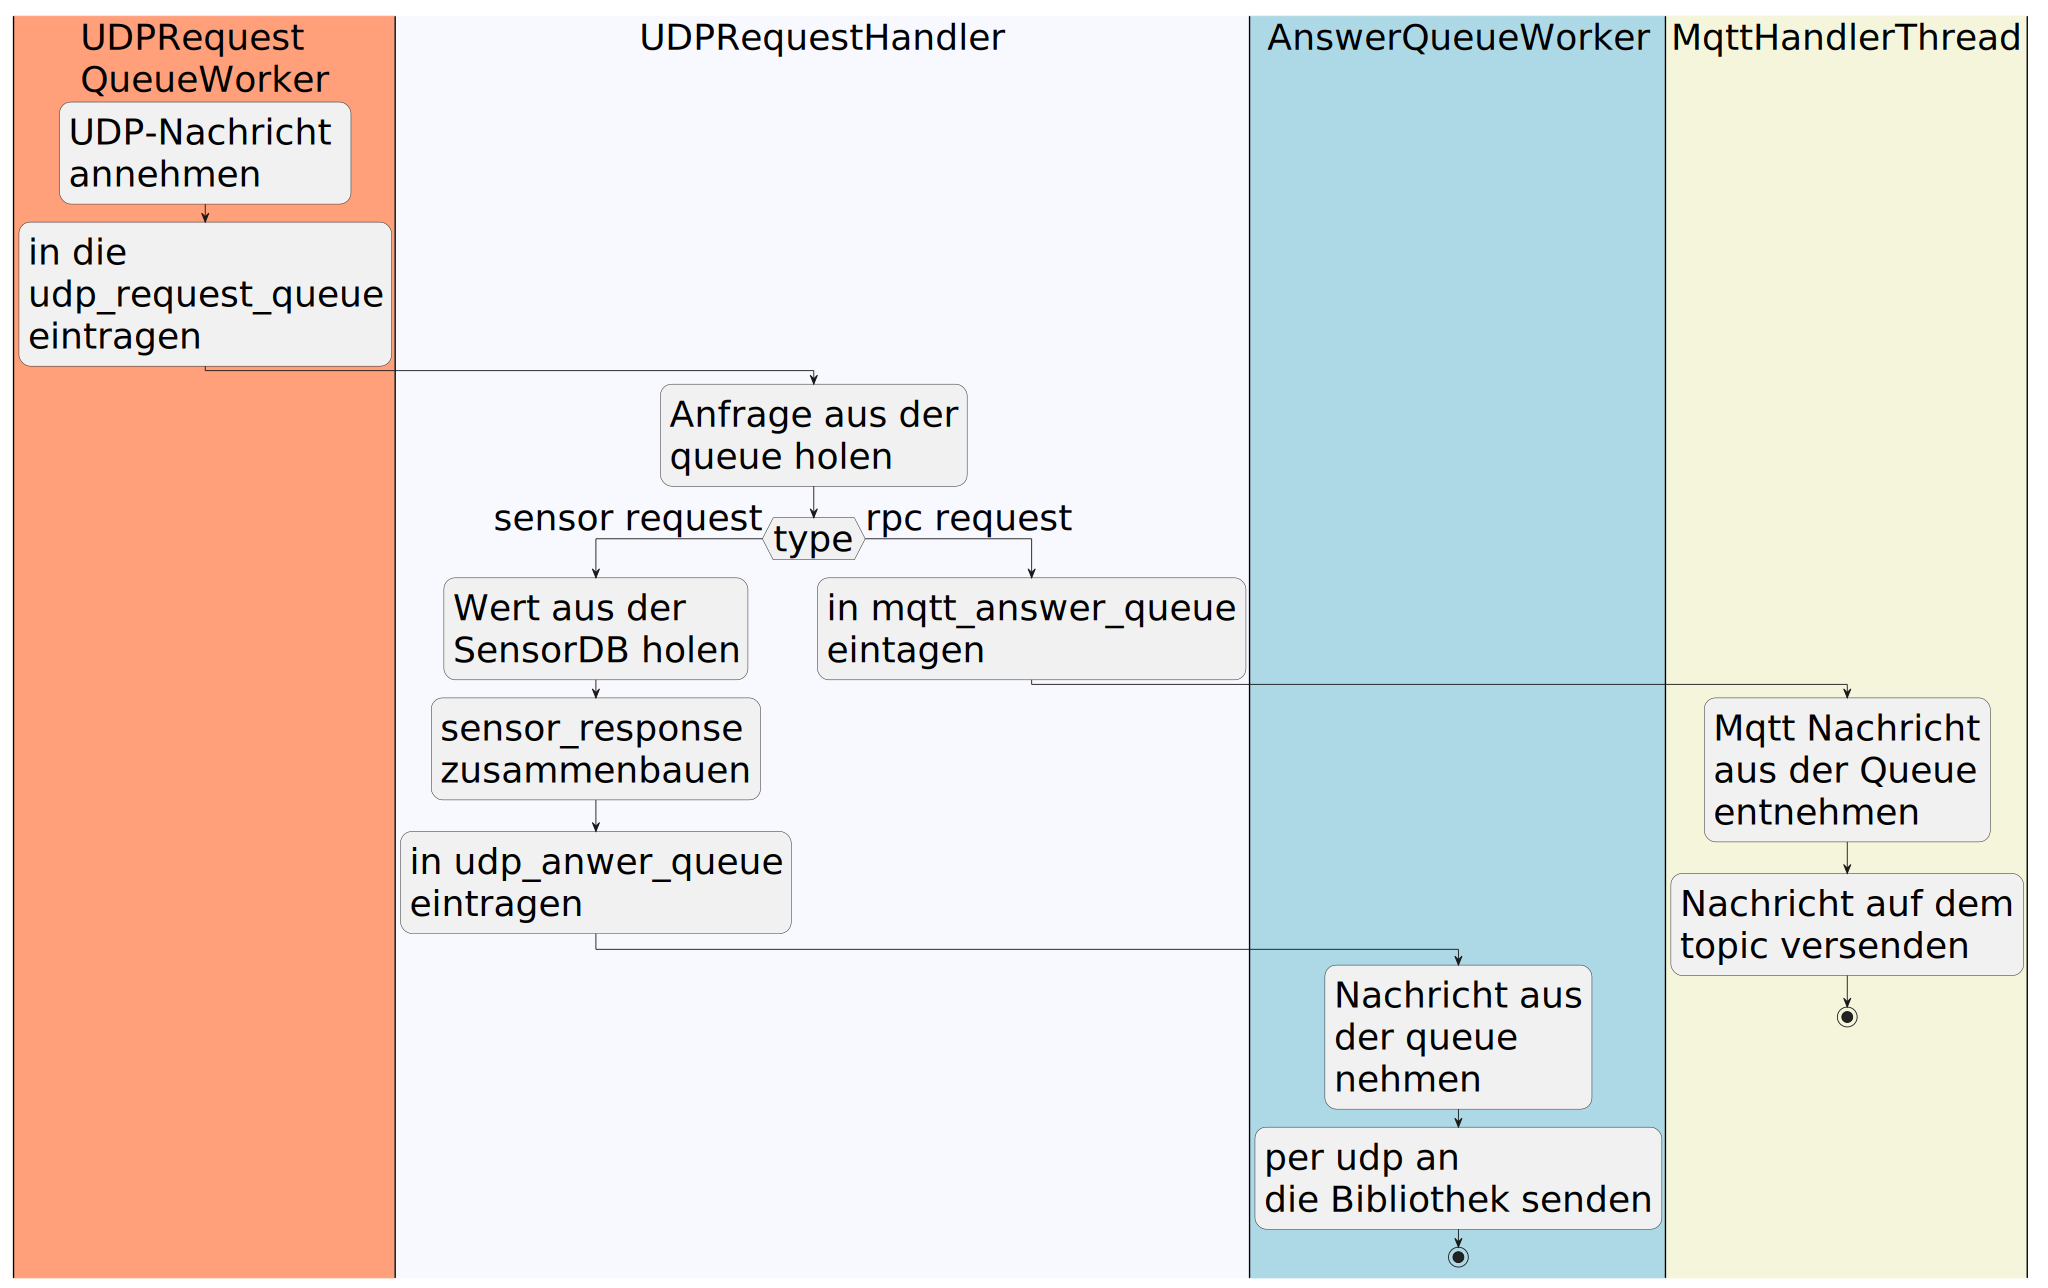
\includegraphics[width=.8\textwidth]{images/UDPRequestServerPath}
  \caption{Ablaufdiagramm UDP Request}
  \label{fig:serverUDPReqPath}
\end{figure}
Erreicht ein UDP Request den Server wird es vom UDPRequestQueue-Worker in eine UDP Request Queue gelegt.
Der UDPRequestHandler-Thread entnimmt die Nachricht und bestimmt den Anfragentyp.
Handelt es sich um eine Anfrage des Types RPC\_Request soll sie Aktionen auf dem Smartphone auslösen.
Sie muss an das Smartphone gesendet werden, was über MQTT möglich ist.
Dafür wird Sie ineine MqttAnswerQueue eingesetzt.
Der MQTTHandlerThread entnimmt Sie und sendet Sie per MQTT ab.
\\
Ist Request hingegen ein SensorRequest, also eine Anfrage auf die ein Sensorwert geantwortet werden soll wird der nachgefragte Sensorwert über die Klasse SensorDB entnommen und in die Udp\_answer\_queue eingetragen.
Der AnswerQueueWorker entnimmt die Anfrage und sendet Sie per udp an die Library zurück.
\\\\
Zusammenfassend erfüllen die Komponenten folgende Aufgaben.
Der MQTTHandlerThread nimmt Nachrichten direkt per MQTT an und gibt die Anfrage weiter.
Außerdem sendet er Nachrichten per MQTT, falls welche anfallen.
\\
Der MQTTRequestHandler kümmert sich um das Verfahren von MQTT Requests.
\\
Der UDPRequestQueue Worker nimmt wie der MQTTHandlerThread Anfragen die per UDP übermittelt wurden an und gibt Sie zur Behandlung entsprechend weiter.
Er sendet jedoch im Gegensatz keine Responses zurück.
\\
Hierfür gibt es den AnswerQueueWorker, dessen einzige Aufgabe es ist Antworten per UDP zurück zu übermitteln.
\\\\
Die Kommunikation zwischen den Threads funktioniert über synchronisierte Queues des queue-Moduls\cite{python_queue} der cpython Implementierung.
Es handelt sich um eine threadsichere Monitorklasse, die einen gleichzeitigen Zugriff zweier unterschiedlicher Threads durch Locks verhindert.

\chapter{Programmierumgebung}\label{chap:libs}
Die Bibliotheken bilden die Einstiegsstelle für Nutzer um die Anwendung fernzusteuern oder Sensorwerte abzufragen.
Funktionsaufrufe liegen jeweils in den Sprachen C, Java und Python vor.
Daten werden wie in Kapitel \ref{chap:architektur} in Abbildung \ref{fig:design} gezeigt per UDP an eine Serveranwendung gesendet.
Diese sendet die Daten dann nach gegebenenfalls per MQTT an das Smartphone weiter, oder wieder per UDP zurück.
\\
Die Bibliotheken senden und empfangen alle jeweils Daten per UDP.
Hierfür werden Sockets benötigt.
Für's Empfangen muss der Socket binded sein.
Die Serveranwendung ist auf dem Port 5006 erreichbar.
Antworten erwarten die Bibliotheken auf dem Port 5005.
\chapter{Evaluation}\label{chap:eval}
\section{Android Anwendung}\label{sec:androidApp}
Für Ausgaben auf dem Smartphone existiert die Android Anwendung Smartbit, die verschiedene Interaktionsmöglichkeiten bereitstellt.
Das Userinterface wird in Abbildung \ref{fig:androidUI} gezeigt.
\begin{figure}[htbp]
  \centering
  \includegraphics[width=.6\textwidth]{images/android_app_ui}
  \caption{Userinterface Android Anwendung}
  \label{fig:androidUI}
\end{figure}
\\
Die Anwendung besteht aus zwei Leds, den beiden Punkten im oberen rechten Eck.
Ein Textfeld in der Mitte kann zur Ausgabe von Text verwendet werden.
Die beiden Buttons können gedrückt werden.
Neben den sichtbaren Elementen kann die Anwendung das Smartphone außerdem vibrieren lassen.



\chapter{Fazit}\label{chap:fazit}
\blindtext

\chapter{Quellen}\label{chap:source}


% Listen wenn überhaupt ans Ende und nicht an den Anfang.
% Meist ist das aber unnötig.
% \listoffigures % Liste der Abbildungen 
% \listoftables % Liste der Tabellen
% \newpage

\bibliographystyle{plain} % Literaturverzeichnis
\begin{btSect}{thesis} % mit bibtopic Quellen trennen
\addcontentsline{toc}{chapter}{Literaturverzeichnis und Online-Quellen}
\section*{Literaturverzeichnis}
\btPrintCited
\end{btSect}
\begin{btSect}{online}
\section*{Online-Quellen}
\btPrintCited
%\bibliography{online}
\end{btSect}
% dann mit "bibtex thesis1" und "bibtex thesis2" arbeiten

\end{document}
;;; Local Variables:
;;; ispell-local-dictionary: "de_DE-neu"
;;; End:


